
%(BEGIN_QUESTION)
% Copyright 2015, Tony R. Kuphaldt, released under the Creative Commons Attribution License (v 1.0)
% This means you may do almost anything with this work of mine, so long as you give me proper credit

\noindent

\vskip 5pt


\textbf{Arbidsoppdrag -- introdusjon}
 I dette oppdraget skal du sjekke at nettverksdokumentasjonen for D426 stemmer. Denne finner i dokumentasjons mappen for D426. 
Du  må sjakke at alle koblinger som vises på kart stemmer og at IP-adressene er slik som  angitt i patchetabellen. 
%$$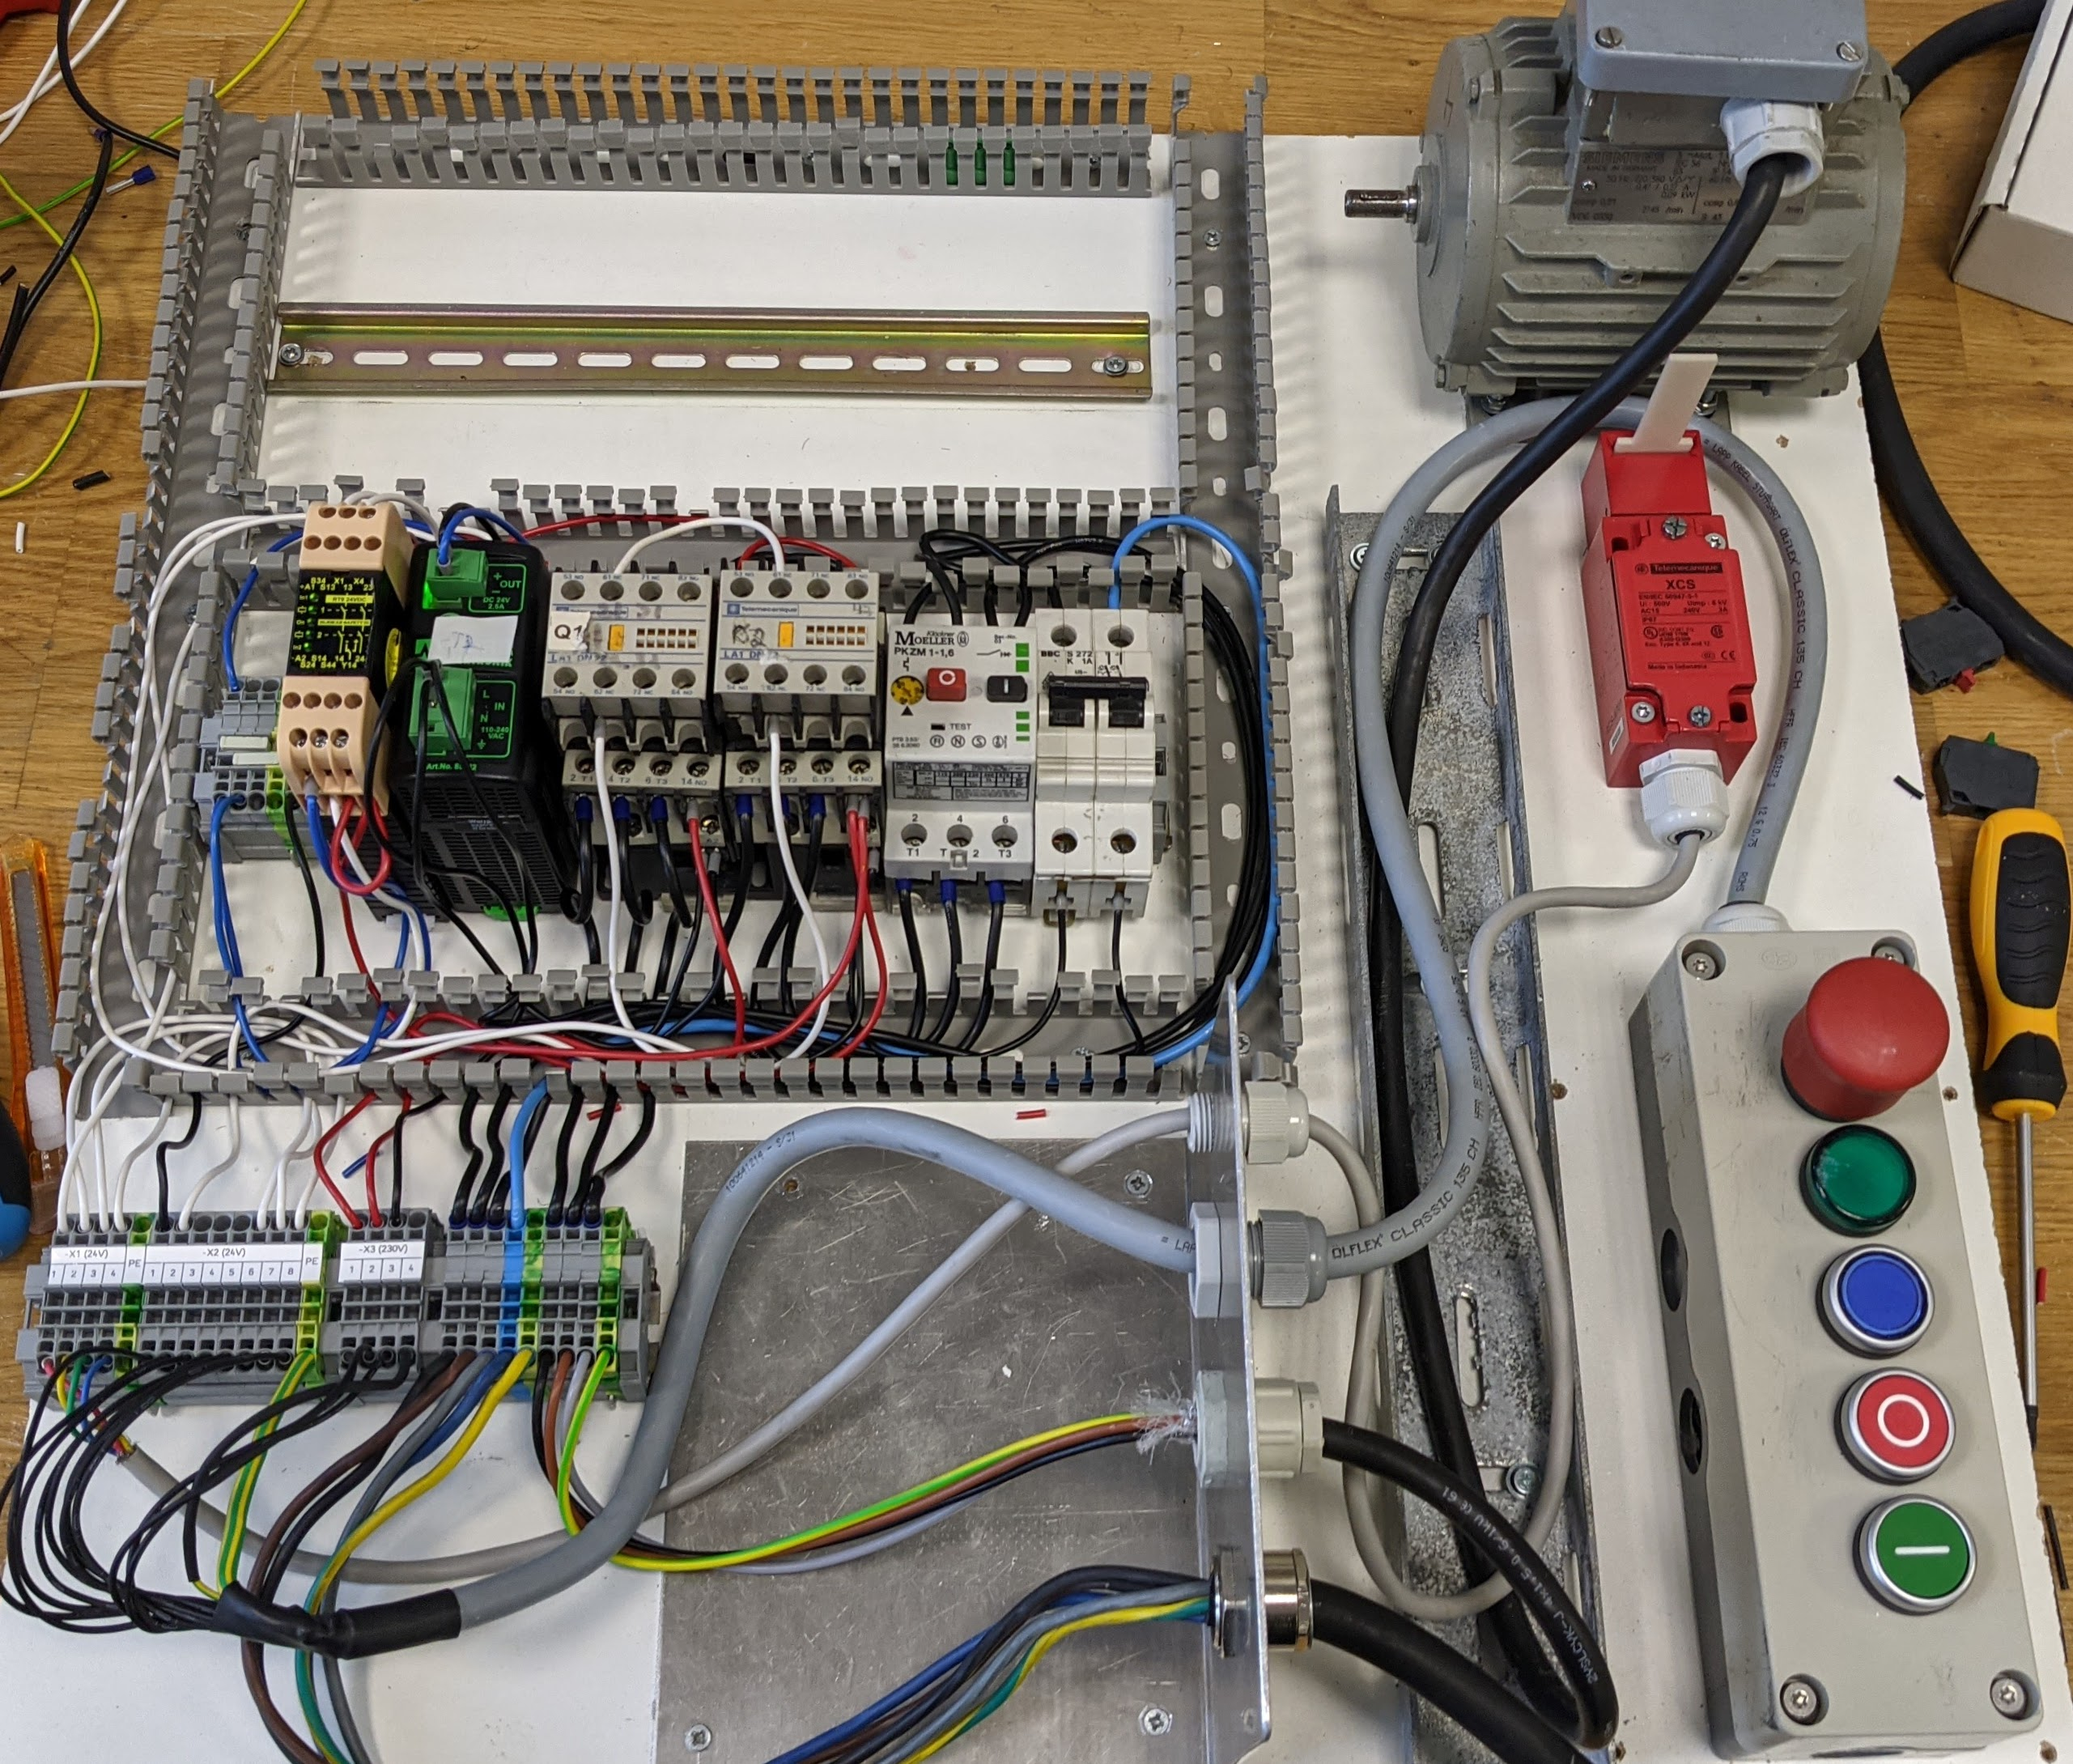
\includegraphics[width=13cm]{i04821x01.jpg}$$\\

\textbf{Teorioppgaver}
\begin{enumerate}



\item Identify the practical purpose of each of these diagnostic utility programs, all accessible through the ``command line'' environment of a personal computer:

\begin{itemize}
\item{} {\tt ping}
\vskip 10pt
\item{} {\tt ipconfig} or {\tt ifconfig}
\vskip 10pt
\item{} {\tt netstat}
\vskip 10pt
\item{} {\tt tracert} or {\tt traceroute}
\vskip 10pt
\item{} {\tt nslookup}
\end{itemize}

Be sure to bring your portable computer to class and experiment with each of these commands!


\item {\it Ethernet} actually encompasses several similar network standards, varying by cable type and bit rate (speed).  The IEEE has designated special identifier names to denote each variety of Ethernet media.  Identify which type of Ethernet each of these names refers to:

\begin{itemize}
\item{} 10BASE2:
\vskip 5pt
\item{} 10BASE5:
\vskip 5pt
\item{} 10BASE-T:
\vskip 5pt
\item{} 10BASE-F:
\vskip 5pt
\item{} 100BASE-TX:
\vskip 5pt
\item{} 100BASE-FX:
\vskip 5pt
\item{} 1000BASE-T:
\vskip 5pt
\item{} 1000BASE-SX:
\vskip 5pt
\item{} 1000BASE-LX:
\end{itemize}

\underbar{file i04466}

\item Each Ethernet device manufactured in the world today possesses a unique identifying number, known as a {\it MAC address} or {\it hardware address}.  This address is 6 bytes, or octets, long (48 bits).  An example of a valid Ethernet MAC address is shown here:

\vskip 10pt

\centerline{\tt D2-48-1C-30-EA-B5}

\vskip 10pt

Given the number of bits in a MAC address field, how many unique identifier addresses can exist in the world?





\item Each Ethernet device manufactured in the world today possesses a unique identifying number, known as a {\it MAC address} or {\it hardware address}.  This address is 6 bytes, or octets, long (48 bits).  An example of a valid Ethernet MAC address is shown here:


\vskip 10pt

\centerline{\tt D2-48-1C-30-EA-B5}

\vskip 10pt

Given the number of bits in a MAC address field, how many unique identifier addresses can exist in the world?





\item This Ethernet network has a problem in it somewhere:


$$\includegraphics[width=15.5cm]{i02123x01.eps}$$

\begin{itemize}
\item{} 1 can ``ping'' 3
\item{} 4 can ``ping'' {\tt www.google.com}
\item{} 4 can ``ping'' 5 
\item{} 2 cannot ``ping'' {\tt www.google.com}
\end{itemize}

\vskip 10pt

An excellent diagnostic strategy is to trace paths of data flow in a complex system, looking for places of intersection.  Successful paths prove all points along the pathway are functioning.  Places of overlap between unsuccessful paths prove that section is suspect.

Apply this strategy to the problem at hand, and use the results to narrow the field of possible faults.

\vskip 10pt

Also, identify a good ``next ping'' test to do.


\underbar{file i02123}



\item The following Ethernet network has a problem.  Someone trying to access the Internet from personal computer \#4 cannot do so, and has called you to troubleshoot the problem:

$$\includegraphics[width=15.5cm]{i04461x01.eps}$$

Your first diagnostic test is to ``ping'' computer \#4 from computer \#5, and you find that this test is successful.  Your next test is to check Internet connectivity at computer \#5 by ``pinging'' {\tt http://www.google.com}, and you find that test is successful as well. 

Identify the likelihood of each specified fault for this network.  Consider each fault one at a time (i.e. no coincidental faults), determining whether or not each fault could independently account for {\it all} measurements and symptoms in this network.

% No blank lines allowed between lines of an \halign structure!
% I use comments (%) instead, so that TeX doesn't choke.

$$\vbox{\offinterlineskip
\halign{\strut
\vrule \quad\hfil # \ \hfil & 
\vrule \quad\hfil # \ \hfil & 
\vrule \quad\hfil # \ \hfil \vrule \cr
\noalign{\hrule}
%
% First row
{\bf Fault} & {\bf Possible} & {\bf Impossible} \cr
%
\noalign{\hrule}
%
% Another row
Hub A failed &  &  \cr
%
\noalign{\hrule}
%
% Another row
Hub B failed &  &  \cr
%
\noalign{\hrule}
%
% Another row
Router failed &  &  \cr
%
\noalign{\hrule}
%
% Another row
Internet service provider failed &  &  \cr
%
\noalign{\hrule}
%
% Another row
Cable failed between computer \#4 and Hub B &  &  \cr
%
\noalign{\hrule}
%
% Another row
Cable failed between Hub A and Router &  &  \cr
%
\noalign{\hrule}
%
% Another row
Cable failed between Hub B and Router &  &  \cr
%
\noalign{\hrule}
%
% Another row
Security settings (e.g. firewall) in computer \#4 &  &  \cr
%
\noalign{\hrule}
} % End of \halign 
}$$ % End of \vbox

Finally, identify the {\it next} diagnostic test or measurement you would make on this system.  Explain how the result(s) of this next test or measurement help further identify the location and/or nature of the fault.

\end{enumerate}


\underbar{file i04461}
\textbf{Planlegging}

\textbf{Gjennomføring}

\textbf{Dokumentasjon}

















\underbar{file i04833}
\vfil \eject
%(END_QUESTION)





%(BEGIN_ANSWER)


%(END_ANSWER)





%(BEGIN_NOTES)


%INDEX% Arbeisdoppdrag, Kompetanse, Nivå 1, Stasjonxx, Mal

%(END_NOTES)


